\documentclass[12pt, letterpaper]{article}
\usepackage{graphicx} %LaTeX package to import graphics
\usepackage[obeyspaces]{url}
\usepackage{hyperref}
\usepackage{subcaption}
\usepackage{listings}



\graphicspath{{images/}} %configuring the graphicx package

\hypersetup{
      colorlinks=true,
      linkcolor=blue,
      filecolor=magenta,      
      urlcolor=cyan,
      pdftitle={Sviluppo di un contatore elettrico intelligente},
      pdfpagemode=FullScreen,
}


\title{
    
\includegraphics[scale=0.5]{unibalogo.jpg}~\\[1cm]
    \textbf{Sviluppo di un contatore elettrico intelligente}
}
\author{Stefano Antonio Labianca}

\date{22 Gennaio 2024 \\[0.125cm] a.a 2023/2024}
\renewcommand*\contentsname{Tabella dei contenuti}
\renewcommand{\figurename}{Figura}
\renewcommand*\refname{}

\begin{document}

\maketitle


\textbf{matricola: } 758364
\hfill
\textbf{email: } s.labianca10@studenti.uniba.it
\hfill \\
\begin{center}
      \textit{Università degli studi di Bari Aldo Moro} \\
      \textit{Caso di Studio per l'esame di Ingegneria della Conoscenza.}
\end{center}


\par\noindent\rule{\textwidth}{0.4pt}~\\[5cm]

\tableofcontents ~\\[5cm]

\section{Introduzione}

Nell'arco della nostra giornata, usiamo diversi dispositivi elettronici e,
alle volte, anche per diverse ore della giornata o addirittura per tutto
il giorno. \\ \break
Per chi abita nelle zone di campagna, o in abitazioni singole, usare molti
dispositivi elettronici contemporaneamente, specialmente se hanno alti consumi o
possiedono una classe energetica bassa, fa scattare il salvavita.

\subsection{Dispositivo salvavita}

Il "salvavita", o più propriamente detto interruttore differenziale, è un dispositivo
che arresta il flusso di energia elettrica dal contatore di
un'abitazione, proteggendo persone e animali. \\ \break
Questi interruttori, monitorano la differenza di corrente in entrata
e in uscita dal dispositivo e, quando la differenza di corrente in entrata e in
uscita supera una certa soglia, allora l'interruttore scatta togliendo l'alimentazione
al circuito.

\begin{figure}
      \centering
      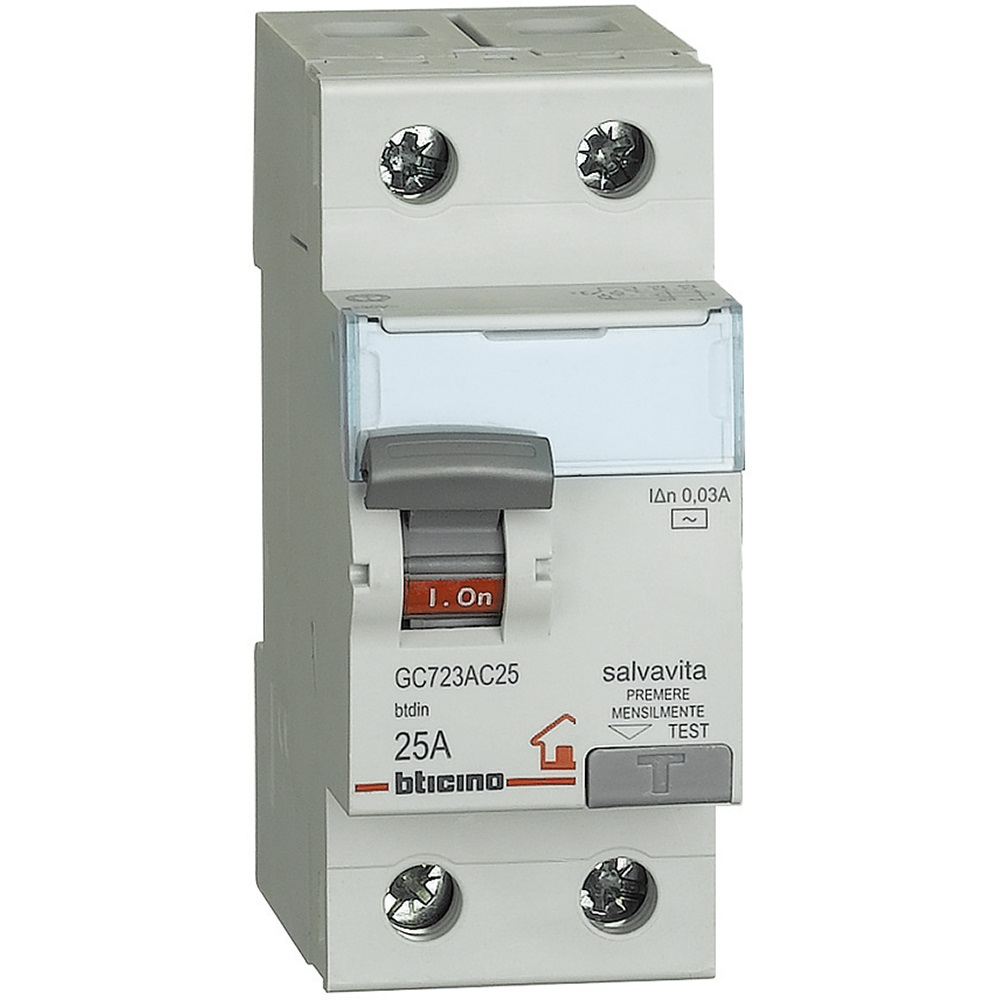
\includegraphics[scale=0.2]{interruttore-diff.jpg}
      \caption{Esempio di contatore differenziale}
\end{figure}


\subsection{Obiettivo del progetto}

Il progetto si pone l'obiettivo di sviluppare un programma in grado di svolgere
i seguenti task:

\begin{enumerate}
      \item Determinare da una lista di dispositivi, quali possono tenere accesi contemporaneamente
            senza che salti il salvavita.
      \item Tenere traccia dei dispositivi elettronici e del loro consumo in Watt.
      \item Ottenere tutti quei dispositivi che rispettano certi vincoli di consumo energetico.
\end{enumerate}

\section{Il progetto}

\subsection{Inizializzare il progetto}

\subsubsection{Scaricare da GitHub}

Il primo passaggio è quello di clonare la repository cliccando al seguente link:
\url{https://github.com/Stefano-Labianca/smart-energy-controller}. \\

\subsubsection{Impostare l'ambiente virtuale}

\noindent Va creato successivamente un ambiente virtuale \cite{create-venv}. In questo modo l'interprete Python,
le librerie e gli script installati al suo interno, saranno isolati dagli altri ambienti
virtuali e da qualsiasi libreria installata sul proprio sistema. \\

\noindent Per creare l'ambiente virtuale, entrate nella cartella del progetto e
digitate il seguente comando:

\begin{verbatim}
      python -m venv .venv
\end{verbatim}

% Mettere citazione nella bibbliografia

\noindent Grazie a questo comando, verrà creata una cartella \path{/.venv} che conterrà tutto il
necessario per lavorare con l'ambiente virtuale. \\

\noindent Una volta creato, è necessario attivare l'ambiente virtuale.
Se siente in ambiente MacOS o Linux, digitate il comando

\begin{verbatim}
      source .venv/bin/activate
\end{verbatim}

\noindent Il file \path{activate} serve per "accendere" l'ambiente virtuale. \\

\noindent Se invece siete in ambiente Windows, allora posizionatevi prima dentro la cartella
\path{./venv/Scripts/} per poi  digitare uno dei seguenti comandi, in base al tipo di terminale in uso:

\begin{verbatim}
      activate.bat // Se usi il CMD
      .\Activate.ps1 // Se usi la PowerShell
\end{verbatim}

\noindent Se invece si sta usando il GitBash, in ambiente Windows, allora il comando da appliace è il seguente:

\begin{verbatim}
      source .venv/Scripts/activate
\end{verbatim}

\noindent L'ambiente virtuale sarà attivato con successo quando sul vostro terminale avrete
qualcosa di simile alla figura 2.

\begin{figure}[h]
      \centering

      \vspace{0.2cm}

      \begin{subfigure}{1\textwidth}
            \centering
            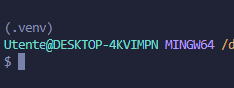
\includegraphics{terminale-bash.png}
            \caption{Uso di GitBash}
      \end{subfigure}

      \vspace{0.3cm}

      \begin{subfigure}{1\textwidth}
            \centering
            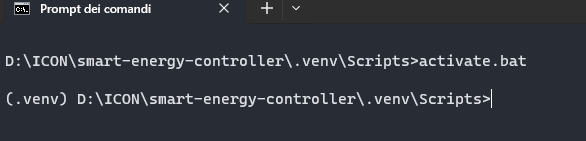
\includegraphics[scale=0.8]{terminale-cmd.png}
            \caption{Uso del CMD}
      \end{subfigure}

      \vspace{0.3cm}

      \begin{subfigure}{1\textwidth}
            \centering
            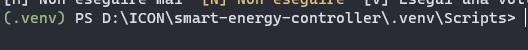
\includegraphics[scale=0.8]{terminale-powershell.png}
            \caption{Uso della PowerShell}
      \end{subfigure}

      \caption{
            Risultato dell'attivazione dell'ambiente virtuale. In figura (a) abbiamo
            l'uso del GitBash, in figura (b) del CMD mentre infine, nella figura
            (c), abbiamo l'uso della PowerShell.
      }
\end{figure} \break

\noindent In caso di problemi nell'uso della PowerShell, è possibile andare alla
sezione: \hyperref[sec:powershell-error]{Risolvere il problema di esecuzione con la PowerShell}. \\

\subsubsection{Avviare il progetto}

Per avviare il progetto, bisogna tornare alla directory principale del progetto e installare
le dipendenze con il comando: \\

\begin{verbatim}
      pip install -r requirements.txt
\end{verbatim}

\noindent Una volta installate, digitare il seguente comando per avviare il programma

\begin{verbatim}
      python main.py
\end{verbatim}

\noindent In caso di errore, vedere la sezione:
\hyperref[sec:python-error]{Errore di esecuzione del programma Python}.

\subsubsection{Avviare un test}

I test svolti sul programma si trovano tutti nella cartella \path{/project_test}. Se si vuole eseguire un
test, basta aprire un file, contenuto in una delle sotto-cartelle, prendere il suo contenuto e spostarlo
dentro il file \path{test_main.py}, presente nella root del progetto, dove si potrà eseguire il testo scelto.

\subsection{Struttura del progetto}

All'intero del progetto, possiamo trovare le seguenti cartelle:
\begin{itemize}
      \item \path{/.vevn}: Cartella contenente tutto il necessario per lavorare con
            l'ambientevirtuale.
      \item \path{/appliance}: Qui è possibile trovare la classe Appliance, che definisce
            un elettrodomestico, insieme ad una serie di metodi di suppporto,
            contenuti in \path{appliances_controller.py}. Insieme ad essi, si trovano dei file csv
            usati per i test del programma.

      \item \path{/cli}: Troviamo una classe che incapsula tutta la logica legata agli input
            e all'output del terminale.

      \item \path{/csp_problem}: Questa cartella contiene tutti i file legati all'argomento del
            CSP. \\
            Infatti è possibile trovare la rappresentazione delle variabili e dei vincoli, fatta
            rispettivamente usando le classi Variable e Constraint. \\
            Inoltre è presente anche la classe CSP usata come wrapper per rappresentare un generico
            problema di questa categoria. \\
            Infine è presenta la cartella \path{/algorithm} che contiene le realizzazioni degli
            algoritmi DFS e GAC usati per risolvere i problemi legati al CSP.

      \item \path{/docs}: In questa cartella è possibile trovare la relazione, in formato PDF, del
            progetto.

      \item \path{/knowledge_base}: Contiene una classe usata per rappresentare il sistema esperto
            realizzato.

      \item \path{/ontology}: Questa cartella contiene una classe che permette di manipolare
            l'ontologia contenuta all'intero del file \path{appliance_ontology.rdf}.

      \item \path{/project_test}: Contiene tutti quei file contenente vari test fatti al programma.

      \item \path{/utils}: Contiene file di utilità che facilitano alcune operazioni interne al programma.
            Per esempio, il file \path{pagination.py} viene usato per impaginare l'output del programma.
\end{itemize}

\subsection{Scelte progettuali}

Il progetto è stato svolto usando le versioni \texttt{3.11.5} e \texttt{3.12.0} di Python in quanto offre diversi
miglioramenti e un supporto maggiore alla tipizzazione delle variabili e delle constanti.
Usare i tipi, infatti, si è rivelato molto utile per rendere la codebase più resiliente, evitando di
assegnare, erroneamente, valori con tipo non corretto per una variabile. \\

\noindent L'uso del design pattern del Singleton si è rivelato utile in quando permette l'uso di
una sola istanza globale della classe \texttt{ApplianceOntology}. Questa classe è stata usata per
rappresentare le informazioni dell'ontologia usata e di manipolarla, tramite operazioni di lettura e
scrittura. \\

\noindent L'istanza creata, infatti, viene usata in più parti del programma e, creare istanze differenti
fra i vari moduli, rischieremmo di avere istanze non aggiornate ai cambiamenti fatti in altre parti del
programma. \\

\noindent Un'altra scelta è stata quella di impaginare \cite{pagination} i risultati dati dagli algoritmi del CSP.
Grazie ad essa, è possibile  dividere grandi quantità di dati in blocchi di dimensioni più piccoli e maneggevoli,
permettendo anche di scorrere una pagina alla volta. \\

\noindent Infine per l'argomento del CSP \cite{ai-python-csp}, sono state usate delle versioni leggermente modificate degli
algoritmi DFS e GAC fornite dal libro di testo AIPython, in quando si è scelto di adattarle al problema
imposto dal progetto. Non solo, lo stesso vale per le classi \texttt{Variable} e \texttt{Contraint} dove sono
stati presi in considerazione solamente le funzionalità essenziali.


\section{Argomenti trattati}

\subsection{CSP}

\subsubsection{Descrizione generale}

Un Constraint Satisfaction Problem, o CSP, si pone l'obiettivo di trovare un insieme di assegnamenti totali che
rispettano dei vincoli. Ogni assegnamento totale, che rispetta i vincoli dati dal problema,  viene considerato come
una soluzione al problema. \\

\noindent Un CSP è formato dalle seguenti componenti:
\begin{itemize}
      \item Insieme finito di variabili;
      \item Ogni variabile ha un dominio;
      \item Insieme di vincoli;
\end{itemize}

\noindent I problemi che voglio risolveri sono: trovare quali dispositivi possono accendere
contemporaneamente senza superare una certa soglia di consumi, limitare i dispositivi da usare, ...
% TODO Trovare altri impieghi

\subsubsection{Algoritmi utilizzati}

Tra gli algoritmi presi in considerazione, sono:

\begin{itemize}
      \item DFS;
      \item Generalized Arc Consistency;
\end{itemize}

\noindent I due algoritmi, prendono i seguenti approcci. \\

\noindent Il primo vuole rappresentare ogni assegnamento come un albero, dove: la sua altezza è
pari al numeri di variabili che si stanno considerando e ogni nodo viene rappresentato come un
assegnamento ad una variabile. \\

\noindent Il secondo invece, prima di trovare delle soluzioni, crea una rete di archi consistenti.
Un arco $\langle X, c \rangle$, con $X$ una variabile e $c$ un vincolo che ha
scope $\{X, Y_1, Y_2, \dots, Y_n\}$, si dice consistente se: per ogni valore $x$ appartenente al dominio
della variabile $X$, esistono dei valori $y_1, y_2, \dots, y_n$, che appartengono ai domini delle loro
corrispettive variabili $Y_i$, tali che, l'assegnamento \\
$\{X=x, Y_1=y_1, Y_2=y_2, \dots, Y_n=y_n\}$ mi va a soddisfare il vincolo $c$. \\

\noindent Per creare archi consistenti, l'algoritmo andrà ad eliminare, per ogni dominio delle variabili, tutti
quei valori che non soddisfano il vincolo $c$. In altri termini va a ridurre lo spazio di ricerca, prima di
andare a trovare una soluzione. \\

\noindent Inoltre, per aiutare maggiormente la riduzione dello spazio di ricerca, è stato scelto di usare
la tecnica del Domain Splitting. In questo modo, il dominio di una variabile viene diviso in due sottodomini
per poi eliminare, in entrambi i domini, quei valori che rendono inconsistente un arco $\langle X, c \rangle$.

\subsubsection{Analisi delle performance}

I due algoritmi sono in grado di trovare le soluzioni ad una serie di problemi dati. Adesso vogliamo sapere quale
dei due riesce a trovare delle soluzioni in tempi minori medi. \\

\noindent I test sono stati svolti usando un Ryzen 5 3400G, sistema operativo Windows 10 e
versione di Python \texttt{3.12.0}. \pagebreak


\noindent \textbf{Test 1} \\

\noindent Voglio trovare degli assegnamenti in cui i dispositivi, della
categoria Multimedia, non vanno a consumare più di $450W$.

\begin{figure}[h]
      \centering
      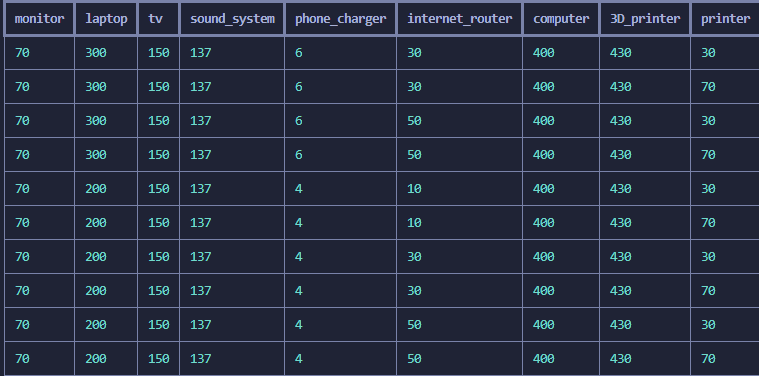
\includegraphics[scale=0.65]{assegnmanenti-dfs.png}
      \caption{Esempio di assegnamenti trovati dal DFS}
\end{figure}

\begin{figure}[h]
      \centering
      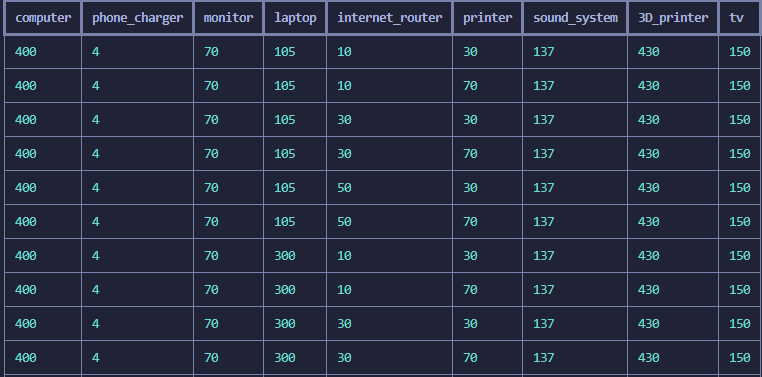
\includegraphics[scale=0.65]{assegnamenti-gac.png}
      \caption{Esempio di assegnamenti trovati dal GAC}
\end{figure}


\break

\noindent Le informazioni sul test sono contenute nel file \path{/appliance/appliance.csv} e
l'esempio mostrato si trova nel file nel \path{/project_test/performance/test_1.py}. \\

\noindent Adesso diamo uno sguardo ai loro tempi di esecuzione. Per farlo vado ad esecuire
entrambi gli algoritmi 10, 100 e 1000 volte, per poi salvare i tempi medi di esecuzione, tramite
la funzione \lstinline|perf_counter_ns()| \cite{perf_counter_ns_docs}. \\

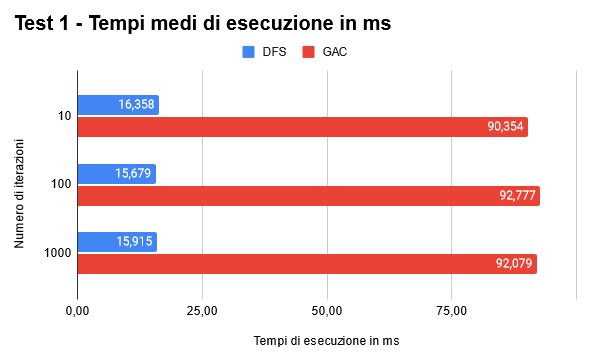
\includegraphics[scale=0.8]{test-1-performance.png}

\noindent Possiamo notare come, nel primo caso di test, l'uso della DFS impiega, in media, molto meno
tempo rispetto al Generalized Arc Consistency. \\ \break

\noindent \textbf{Test 2} \\

\noindent Prendiamo adesso una situazione di un ambiente casalingo, dove possiamo troviamo accesa una
friggitrice, il forno, la televisione, insieme al suo impianto audio, il router, un computer
fisso con il suo monitor, un caricatore del telefono, un frigo, il freezer e l'aspirapolvere.
In questo situazione, non possiamo andare oltre i $3kW$. \\

\noindent Le informazioni sul test sono contenute nel file \path{/appliance/home.csv} e il test dentro
\path{/project_test/performance/test_2.py}. \\

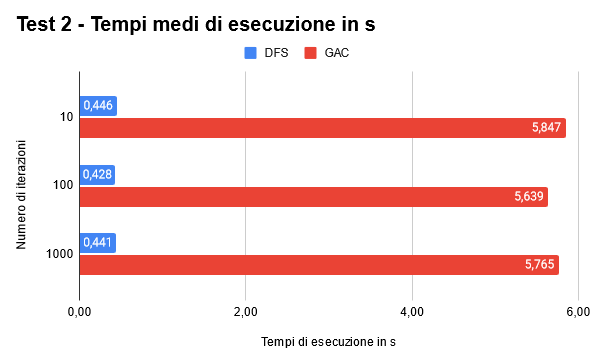
\includegraphics[scale=0.8]{test-2-performance.png}


\subsubsection{Conclusioni}

\noindent Si può evidenziare da questi due test, come l'uso del GAC sia meno conveniente, in termini
di tempo di esecuzione media, rispetto alla DFS. Le motivazioni sono legate alle modalità di ricerca delle soluzioni. \\

\noindent La DFS crea un albero con profondità massima pari al numero delle variabili del problema e, in
caso dovesse trovare un assegnamento parziale che non soddisfa uno o più vincoli, allora usa il
backtraking e inizia a creare una nuova diramazione. \\

\noindent Il Generalized Arc Consistency, invece, va a rimuovere dai domini di ogni variabile, tutti quei valori
che rendono la rete inconsistente. Questo viene fatto andando a dividere il dominio di una variabile in due suoi
sottodomini e, per entrambi, cerca quali valori rendono inconsistente l'arco.
Infine, dopo aver eliminato i valori indesiderati, mi determina tutti gli assegnamenti che risolvono il problema.


\subsection{Ontologie}

\subsubsection{Descrizione generale}

In informatica, un'ontologia è una rappresentazione formale, condivisa che esplicita
una concettualizzazione di un dominio di interesse. In particolare, nell'ampito dell'AI,
è una specifica dei significati dei simboli di un sistema informativo. \\

\noindent Quindi specifica quali individui e relazioni esistono, e quale
terminologia è usata per descriverli.

\subsubsection{Protégé}

Lo strumento utilizzato per creare l'ontologia è Protégé \cite{protege} usando la versione
\texttt{5.6.3}.

\pagebreak

\begin{figure}[h]
      \centering
      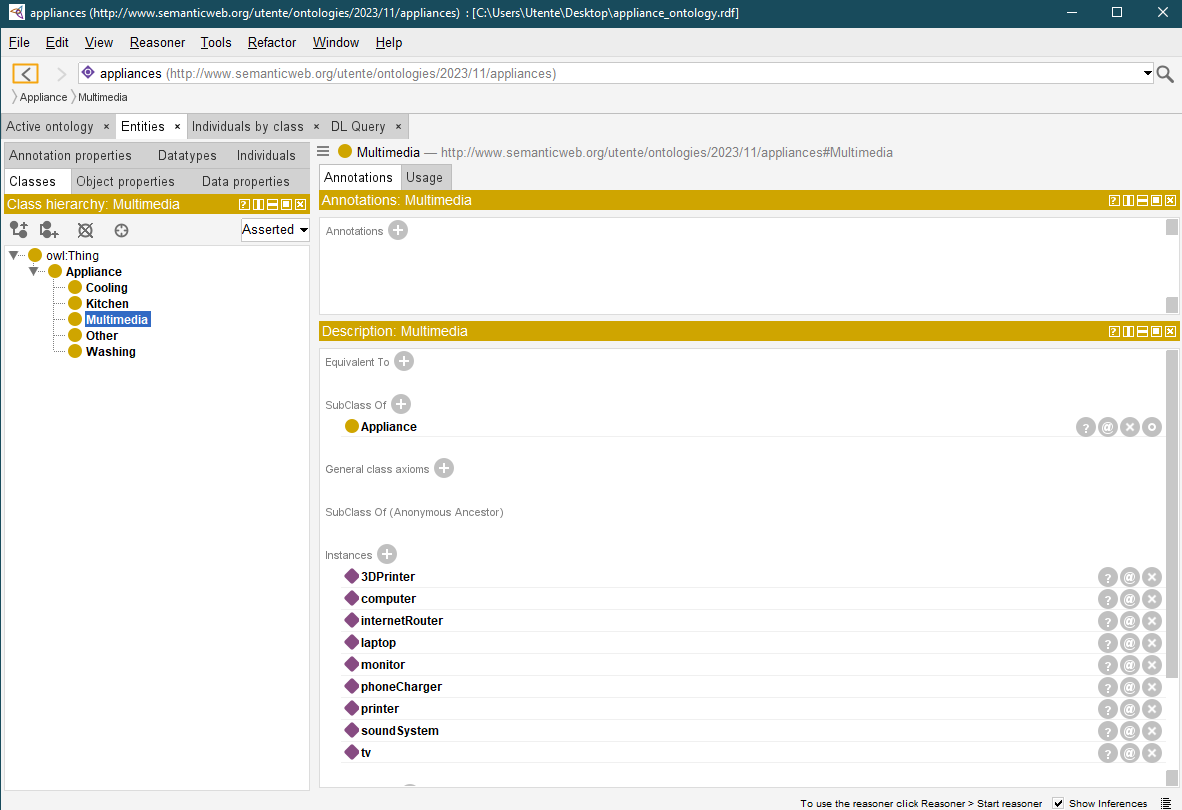
\includegraphics[scale=0.4]{protege-home.png}
      \caption{Schermata del tool Protégé}
\end{figure}

\noindent L'ontologia è organizzata prendendo in considerazione la classe
principale \texttt{Appliance}, usata per rappresentare un generico dispositivo elettronico.
All'interno di essa, sono presenti le seguenti data property:

\begin{itemize}
      \item \path{appliance_name}: Nome del dispositivo;
      \item \path{energy_consumption}: insieme di possibili consumi elettrici per uno stesso
            dispositivo;
      \item \path{size}: Dimensioni del dispositivo. Queste possono
            essere: \texttt{small, medium} oppure \texttt{large};
\end{itemize}

\noindent Le data property sono utilizzate per contenere valori primitivi, come stringhe o interi. \\

\noindent La classe \texttt{Appliance} possiede le seguenti sottoclassi, che andranno ad ereditare i
data property della classe genitore.

\begin{itemize}
      \item \path{Multimedia}: Contiene tutti gli individui che fanno parte della categoria dei dispositivi multimediali.
      \item \path{Kitchen}: Contiene tutti gli individui che fanno parte della categoria dei dispositivi per la cucina.
      \item \path{Cooling}: Contiene tutti gli individui che fanno parte della categoria dei dispositivi legati a rinfrescare
            le strutture abitative.
      \item \path{Washing}: Contiene tutti gli individui che fanno parte della categoria dei dispositivi per la pulizia.
      \item \path{Other}: Contiene tutti gli individui che non fanno parte delle sottoclassi precedenti.
\end{itemize}

\noindent L'uso di queste sottoclassi, ci permette di distinguere meglio la categoria degli individui sfruttando
la proprietà \texttt{rdfs:subClassOf(C1,C2)}, questa infatti mi dice che la
classe \texttt{C1} è sottoclasse di \texttt{C2}. \\

\noindent Tra gli individui, infatti, oltre ad assegnare dei valori alle data property, assegno come tipo la sua
sottoclasse di appartenenza.

\begin{figure}[h]
      \centering
      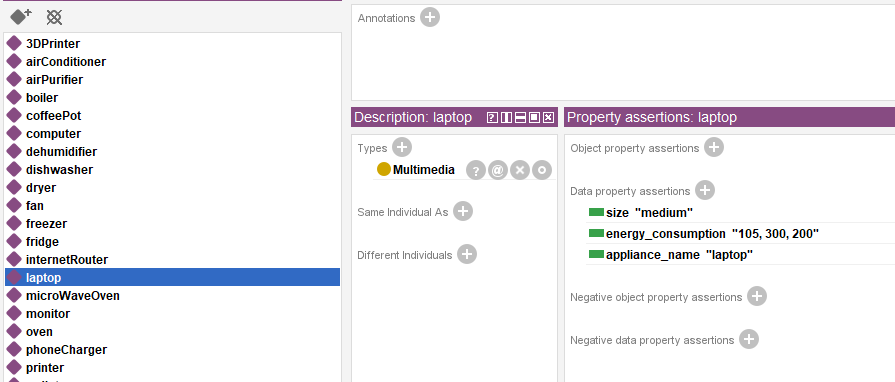
\includegraphics[scale=0.6]{individui-protege.png}
      \caption{Schermata degli invidui, con assegnamento dei valori alle sue proprietà e tipo.}
\end{figure}

\subsubsection{Lavorare sull'ontologia}

Per lavorare sull'ontologia, ho usato la libreria \texttt{rdflib}. Grazie ad essa, è stato possibile
caricare il file \path{/ontology/appliace_ontology.rdf} e di applicare su di esso una serie di operazioni, come:

\begin{itemize}
      \item Lettura dell'ontologia;
      \item Ricerca di un individuo;
      \item Verificare la presenza di un individuo;
      \item Rimuovere un individuo;
      \item Aggiungere un individuo;
\end{itemize}

\noindent I dati contenuti nell'ontologia, vengono usati per strutturare i dispositivi elettronici e, una volta
letti, vi è possibile applicare gli algoritmi di CSP o usare il sistema esperto.

\subsection{Sistema esperto}

\subsubsection{Descrizione generale}

\noindent Un sistema esperto è un programma che cerca di riprodurre le prestazioni di una o più
persone esperte in un determinato campo. \\

\noindent Un sistema esperto si basa sull'uso di una base di conoscenza, ovvero un insieme
di assiomi veri. Ogni assioma della base di conoscenza è una clausole definite del tipo:

\[ h \leftarrow a_1 \land  a_2 \land \dots \land a_m \]

\noindent dove sia $h$ che ogni $a_i$ sono atomi.

\noindent $h$ viene detta testa della clausola, mentre
$a_1 \land  a_2 \land \dots \land a_m$ è il corpo della clausola. \\

\noindent In base al numero di atomi presenti nel corpo della clausola, possiamo dividerle in due categorie:
\begin{itemize}
      \item Se $m > 0$, allora la clausola viene chiamata \textit{regola};
      \item Se $m = 0$, allora la clausola viene chiamata \textit{fatto};
\end{itemize}

\noindent Il sistema esperto sviluppato, si pone l'obiettivo di segnalare all'utente
se i dispositivi che vuole usare, possono portare a far scattare il salvavita. \\


\subsubsection{Realizzazione del sistema esperto}

Il sistema esperto possiede una serie di fatti, ovvero il consumo elettrico di tutti dei dispositivi
presenti nell'ontologia. Per realizzarli, è stata usata la libreria Experta, una libreria Python, dove le regole
si basano su due idee:

\begin{itemize}
      \item LHS (Left Hand Side): Definisce le condizioni che devono essere verificate affinché la regola
            sia verificata;
      \item RHS (Right Hand Side): Le operazioni eseguite quando la regola viene applicata;
            sia verificata;
\end{itemize}

\noindent Un esempio di regola è la seguente:

\begin{lstlisting}[language=Python]
    @Rule(Fact(action="start")) # LHS
    def start_system(self):
        # RHS


\end{lstlisting}

\noindent In altri termini: LHS è il decoratore \texttt{@Rule()}, che si trova
sopra la definizione di un metodo, mentre l'RHS sono le istruzioni che quel metodo
eseguirà quando la regola sarà applicata. \\

\noindent Le regole utilizzate sono le seguenti, che si differenziano in base allo stato
del sistema:

\begin{itemize}
      \item \path{status_up}: Il salvavita non salterà;
      \item \path{status_warning}: Il salvavita potrebbe salterare a causa di improvvisi
            picchi nell'uso del dispositivo elettronico che consuma di più;
      \item \path{status_down}: Il salvavita scatterà;
\end{itemize}

\noindent Ad ognuno di esse è stata assegnata un metodo Python della classe \\
\texttt{ExpertSystem} e, in caso si ritrovi nello stato \path{status_warning} o \path{status_down}, il sistema esperto avviserà l'utente
dello stato, andandoli a consigliare quale dispositivo deve essere spento oppure quale va limitato l'uso.

\subsubsection{Funzionamento}

\noindent Per avviare il sistema esperto, viene richiamata la funzione \\
\path{run_expert_system(max_usage: float)}, dove il parametro richiesto è il limite del salvavita espresso in $kWh$. \\

\noindent Il sistema esperto, una volta avviato, andrà a chiedere all'utente quali dispositivi elettronici vuole
accendere.

\begin{figure}[h]
      \centering
      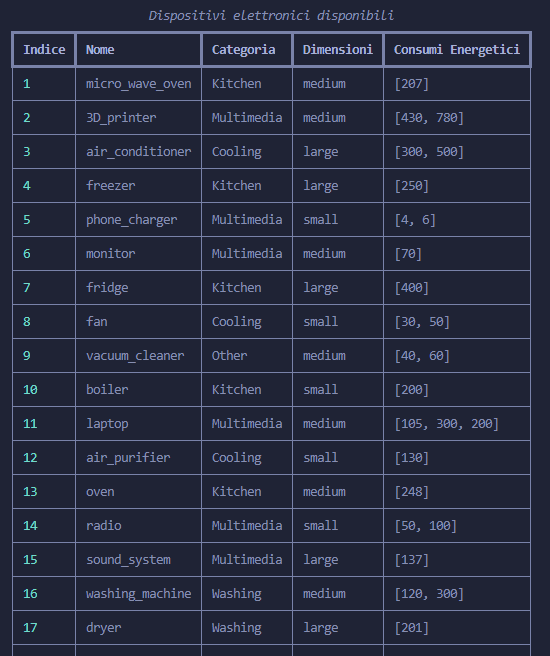
\includegraphics[scale=0.8]{dispositivi-tabella.png}
      \caption{Alcuni dispositivi disponibili.}
\end{figure}

\noindent Una volta selezionati i dispositivi da controllare, se un dispositivo ha più consumi energetici,
verrà chiesto quale deve prendere in considerazione.


\begin{figure}[h]
      \centering
      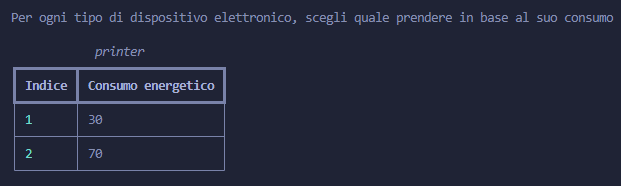
\includegraphics[scale=0.8]{printer-choose.png}
      \caption{Esempio di scelta di un dispositivo}
\end{figure}

\noindent Infine, una volta scelti, il sistema esperto determina se non faranno saltare il
contatore, andando a simulare per un'ora l'uso dei dispositiv scelti. \\ \\
Mostriamo alcuni esempi, realizzati considerando come soglia massima \\ $1.7kWh$. \\

\noindent \textbf{Esempio 1}

\noindent Seleziono solamente una stampate da $70W$

\begin{figure}[h]
      \centering
      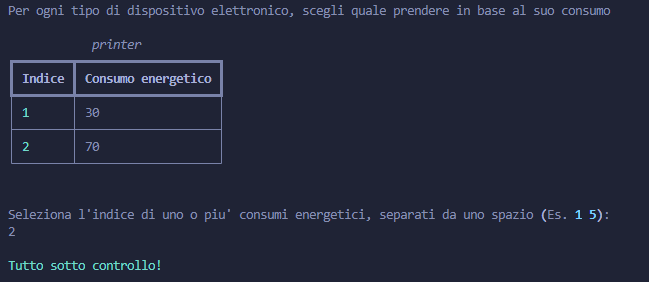
\includegraphics[scale=0.70]{sistema-esperto-esempio-1.png}
      \caption{Primo esempio di uso del sistema esperto}
\end{figure}

\noindent \textbf{Esempio 2}

\noindent Adesso scegliamo una TV da $150W$, il suo impianto audio da $137W$, condizionatore da $500W$ e una
stampate 3D da $780W$.

\begin{figure}[h]
      \centering
      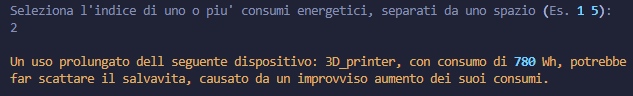
\includegraphics[scale=0.70]{sistema-esperto-esempio-2.png}
      \caption{Secondo esempio di uso del sistema esperto}
\end{figure}

\noindent La soglia per cui viene mostrato questo messaggio è di $150W$, infatti se la differenza del
consumo massimo consentito e la somma dei dispositi scelti, non supera i $150W$ allora il salvavita potrebbe
saltare. \\

\noindent \textbf{Esempio 3}

\noindent Adesso scegliamo un condizionatore da $500W$, una stampate 3D da $780W$, una
lavatrice da $300$ e il frigo da $400W$.

\begin{figure}[h]
      \centering
      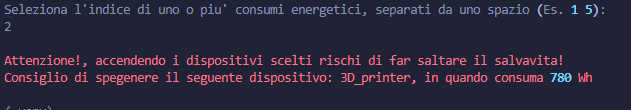
\includegraphics[scale=0.8]{sistema-esperto-esempio-3.png}
      \caption{Terzo esempio di uso del sistema esperto}
\end{figure}


\section{Troubleshooting}

\subsection{Risolvere il problema di esecuzione con la PowerShell}
\label{sec:powershell-error}

In caso non si riesca ad eseguire con la PowerShell \cite{power-shell-resolution},
l'attivazione dell'ambiente virtuale, provate a svolgere i seguenti passi. \\

\noindent Aprire innanzitutto la PowerShell come amministratore nella cartella del progetto.
Una volta aperta la PowerShell, digitare il comando:

\begin{verbatim}
      Get-ExecutionPolicy
\end{verbatim}

\noindent Grazie a questo comando, possiamo sapere quale execution policy è impostata per la PowerShell.
Nella figura seguente, è mostrato una possibile execution policy impostata nella PowerShell. \\

\begin{figure}[h]
      \centering
      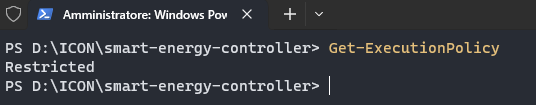
\includegraphics{powershell-error.png}
      \caption{Possibile execution policy}
\end{figure}

\noindent Per permettere l'esecuzione degli script \texttt{.ps1}, allora bisogna impostare
su \texttt{AllSigned} la execution policy. \\
\noindent Per farlo si usa il comando: \\

\begin{verbatim}
      Set-ExecutionPolicy -ExecutionPolicy AllSigned
\end{verbatim}

Una volta eseguito questo comando, andare nella cartella \path{/.venv/Scripts/} e digitare il
comando:

\begin{verbatim}
      .\Activate.ps1
\end{verbatim}

Apparirà sul terminale il seguente output: \\

\begin{figure}[h]
      \centering
      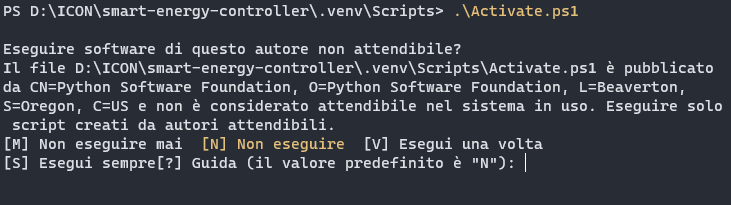
\includegraphics[scale=0.6]{terminal-message.png}
      \caption{Messaggio di conferma}
\end{figure}

Per eseguire lo script di attivazione, allora inserite \texttt{V} e
premete invio. \\ \break

\noindent Una volta che avete finito l'esecuzione del programma, potete anche reimpostare
la execution policy al suo stato precedente, usando il comando:

\begin{verbatim}
      Set-ExecutionPolicy -ExecutionPolicy <PolicyNamePrecedente>
\end{verbatim}


\subsection{Errore di esecuzione del programma Python}
\label{sec:python-error}

E' possibile che, durante l'esecuzione del programma, possa apparire il seguente
messaggio di errore \cite{python-mapping-problem}:

\begin{figure}[h]
      \centering
      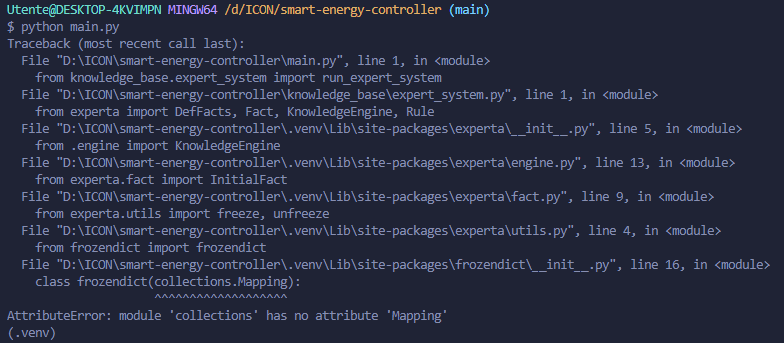
\includegraphics[scale=0.55]{errore-python.png}
      \caption{Errore di esecuzione}
\end{figure}

\noindent Questo errore è dovuto ad una versione datata della libreria \texttt{frozendict}
usata come dipendenza della libreria \texttt{experta}. \\

\noindent Fare l'upgrade della libreria \texttt{frozendict} alla versione più recente, andrebbe a
creare dei conflitti di dipendenza tra le due versioni della librerie. \\

\noindent Per risolvere questo problema, bisogna andare nella cartella
\path{/.venv/Lib/site-packages/frozendict} e aprire il file \path{__init__.py}.

\noindent Una volta aperto, bisogna cambiare la seguente linea di codice: \\

\begin{lstlisting}[language=Python]
      class frozendict(collections.Mapping):
            ...
\end{lstlisting}

Nella seguente:

\begin{lstlisting}[language=Python]
      class frozendict(collections.abc.Mapping):
            ...
\end{lstlisting}

\section{Conclusioni e Sviluppi Futuri}

L'applicativo realizzato, è riuscito nell'intendo di poter tenere traccia degli elettrodomestici
presenti, di poter fornire feedback all'utente su quale dispositivo rischia di far saltare il salvavita
e, infine, di poter determinare quali dispositivi rispettino i vincoli forniti. \\

\noindent Possiamo estendere e migliorare l'applicativo in vari modi:
\begin{itemize}
      \item Migliorare l'interazione con l'utente tramite una GUI;
      \item Avviare una simulazione dell'uso di un sottogruppo di elettrodomestici
            nell'arco di una giornata per un individuo;
      \item Poter considerare, insieme al consumo energetico, anche i costi della bolletta;
      \item Uso di dataset che prendano in considerazione consumi e tempi di utilizzo reali;
      \item Espandere la base di conoscenza, con il costo energetico di ogni dispositivo elettronico;
\end{itemize}

\section{Riferimenti Bibliografici}

\begin{thebibliography}{100}
      \bibitem{create-venv}
      freeCodeCamp (2022):  \href{https://www.freecodecamp.org/news/how-to-setup-virtual-environments-in-python/}{
            Creazione di un ambiente virtuale in Python.
      }

      \bibitem{pagination}
      Paginazione: \href{https://www.educative.io/answers/what-is-pagination}{
            Funzionamento della paginazione.
      }

      \bibitem{ai-python-csp}
      AIPython (2023): \href{https://artint.info/AIPython/aipython/aipython.pdf}{
            Ragionamento con i vincoli, capitolo 4 pagina 69.
      }

      \bibitem{perf_counter_ns_docs}
      \lstinline|perf_counter_ns()|: \href{https://docs.python.org/3/library/time.html#time.perf_counter_ns}{
            Documentazione ufficiale per la funzione \lstinline|perf_counter_ns()|.
      }

      \bibitem{protege}
      Protégé: \href{https://protege.stanford.edu/}{Sito ufficiale di Protégé.}


      \bibitem{power-shell-resolution}
      PowerShell Documentation (2022):
      \href{https://learn.microsoft.com/en-gb/powershell/module/microsoft.powershell.core/about/about_execution_policies?view=powershell-7.4}{
            Documentazione sul funzionamento delle execution policy della PowerShell Windows.
      }

      \bibitem{python-mapping-problem}
      Attribute Error (2023): \href{https://stackoverflow.com/questions/70749690/attributeerror-module-collections-has-no-attribute-mapping}{
            Risoluzione problema legato alle dipendenze datate.
      }


\end{thebibliography}

\end{document}